\documentclass{article}
\usepackage[a4paper, portrait, margin=1cm, right=1cm]{geometry}
\usepackage{fontspec}
\usepackage[fleqn]{amsmath}
\usepackage{setspace}
\usepackage{graphicx}

\graphicspath{./graphics/}
\setmainfont[Ligatures=TeX]{Linux Libertine}

\title{Информационные технологии. Лекция 02. Свойства КФС. Основные компоненты КФС.}
\author{Студент группы 2305 Макурин Александр}
\date{13 февраля 2023}

\begin{document}
\maketitle
\begin{sloppypar}
    \setstretch{1.8}

    \section{Свойства КФС}
    \subsection{Имманентные}
    Свойственны любой КФС

    Связь

    Механика

    Анализ окружающей среды

    \subsection{Трансцендентные}
    Зависят от реализации

    Перемещение

    Целевая нагрузка

    Взаимодействие с оператором (?)

    \section{Архитектура (делиберативная/реактивная):}
    В зависимости от типа КФС меняются:
    \begin{itemize}
        \item Цель (идеальное функционирование/$e_i^t \rightarrow e_i^{t - 1}$ или стабильность)
        \item Критерии (есть/нет)
              $R = <r_1, ..., r_n>$ - все ресурсы системы. $r_1$ соответствует $e_1$.

              Достижение перечня задач:
              \[
                  \left\{\begin{array}{ll}
                      |TK^e| \rightarrow |TK| \\
                      cost(TK) \leq R
                  \end{array}\right.
                  \text{ где $cost$ - затраты}
              \]
        \item Стратегии (есть/нет)
              \[
                  \left\{\begin{array}{ll}
                      |TK^{ei}| \rightarrow |TK| \\
                      cost(TK^{ei}) \leq R^{ei}
                  \end{array}\right|
                  - \text{ каждый сам пытается достичь целей}
              \]

              Отличие между индивидуальным и групповым достижением целей:

              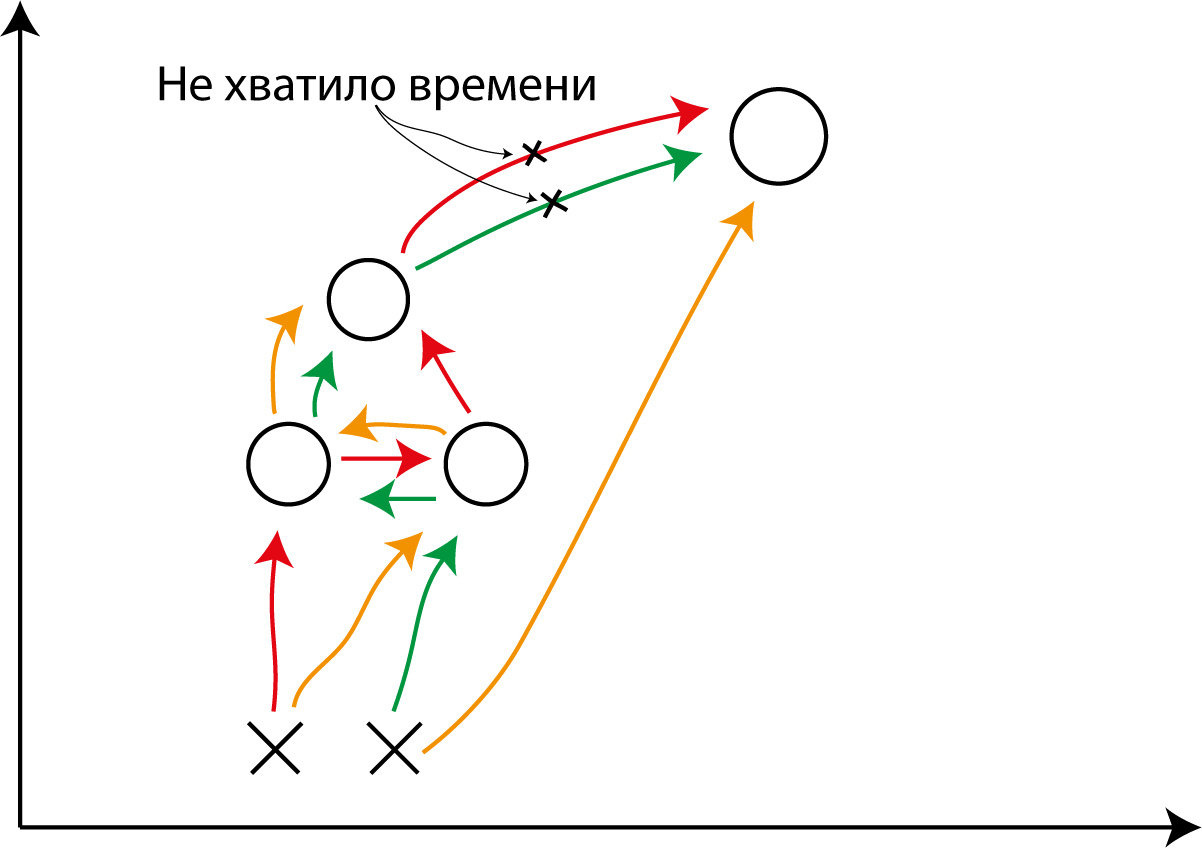
\includegraphics[width=0.6\textwidth]{graphics/Два сценария достижения цели.png}

              Круги - цели, кресты - субъекты, стремящиеся к их достижению.
              Красные и зелёные линии обозначают случай с индивидуальной попыткой достижения целей, оранжевые - групповую попытку.

              В качестве примера можно привести выполнение студентами лабораторных работ. По одиночке успеть сделать все невозможно, но, разделив работы, получение автомата становится вполне реальным.

        \item Взаимодействие ((есть или косвенное)/(нет или косвенное))
        \item Память
              \[
                  S^{t + 1} = F(E^t, U^t, {S^{t}})
              \] - делиберативная c памятью
              \[
                  S^{t + 1} = F(E^t, U^t)
              \] - делиберативная
              \[
                  S^{t + 1} = F(U^t)
              \] - реактивная
    \end{itemize}

    \subsection{4 функции любой системы:}
    \begin{itemize}
        \item Сбор
        \item Хранение
        \item Обработка
        \item Передача
    \end{itemize}

    \subsection{3 уровня связи}
    \begin{itemize}
        \item Физ $\rightarrow$ инф
        \item Инф $\rightarrow$ физ
        \item Инф $\rightarrow$ инф
    \end{itemize}

    $|W_{phy}| = const$

    $|W_{inf}| \rightarrow \infty$

    Канал связи принимаем условно идеальным ($P_{\text{передачи}} = 1$)

    Источник $\rightarrow$ канал ($\varepsilon$) $\rightarrow$ прёмник

    DJI являются лучшими беспилотниками, потому что канал передачи на нём идеальный (всё на одной плате, нет проводов-"шнурков")

    $B$ - пропускная способность канала

    $M$ = $U_{in_i}$ - множество сообщений

    $t_{\text{пер}} = \dfrac{M}{B}$ - время передачи

    $t_{пр. р.} = 2\alpha_1t_{\text{пер}} + \alpha_2t_{\text{формирования плана}} + \delta$, где $\delta$ - время выполнения плана, $\alpha_2$ - сложность формирования плана (зависит от оптимальности алгоритма), $\alpha_1$ - шум

    Управляемые нами параметры (на которые мы можем влиять):
    \begin{align*}
         & B \rightarrow max \text{(нас интересует)}      \\
         & M \rightarrow min                              \\
         & \alpha_1 \rightarrow 1 \text{(нас интересует)} \\
         & \alpha_2 \rightarrow 0
    \end{align*}

    ЛПР (лицо принимающее решение)
    $Per : e_i \rightarrow S^{per}$, $Per$ - функция оценки, $e_i$ - элемент кибернетической системы, $S^{per}$ - субъективное представление об элементе

    $S$ - пространство $\forall$ (любых) состояний системы $E$.

    В контексте КФС $\overline{S^t} = S^t + \epsilon$, где $\overline{S^t}$ - мнение наблюдателя о системе, $S^t$ - реальное состояние $\epsilon$ - погрешность.

    \begin{itemize}
        \item $e_i \neq e_j \Leftrightarrow Per(e_i) \neq Per(e_j)$
        \item $\forall e_i \exists S^{per}_{ei}$
    \end{itemize}
    $\lim S_{ei}^{per} = S_{ei}$

    $\Delta S \rightarrow \infty$ - мы ничего не знаем о системе

    Варианты связи с наблюдаемостью:
    \begin{itemize}
        \item $y(t) \rightarrow 0$ - нет данных (система спит/мертва)
        \item $Per(y(t)) \rightarrow 0$ - данные есть, но наблюдатель ничего
              не понял (наблюдатель спит/мёртв)
        \item $|Per(y(t))| - |y(t)| \rightarrow 0$ - наблюдатель что-то понимает о каком-то элементе системе (количественное сравнение)
        \item $Per^* - \lim Per(y(t)) = Per^*$ - качественное сравнение
    \end{itemize}

    В рамках курса ЛПР=СУ (система управления).

    В контексте инф-инф:

    источник - кодировщик - канал связи (шум) - декодировщик - приёмник

    $P_{\text{приёма}} \rightarrow 0 \Leftrightarrow \text{шум} \rightarrow \infty$



\end{sloppypar}
\end{document}